\chapter{Classificatori Poselets} \label{cap2}
In questo capitolo viene presentato il procedimento per ottenere i classificatori relativi ai 4 tipi di poselets presi in considerazione. Successivamente vediamo come vengono raggruppate le attivazioni-poselet per ottenere il bounding box della persona.

\section{Addestramento Classificatore Poselet}
Il procedimento per l'addestramento dei Classificatori Poselet è raffigurato in \ref{class-pos}

\begin{figure}[h]
\centering
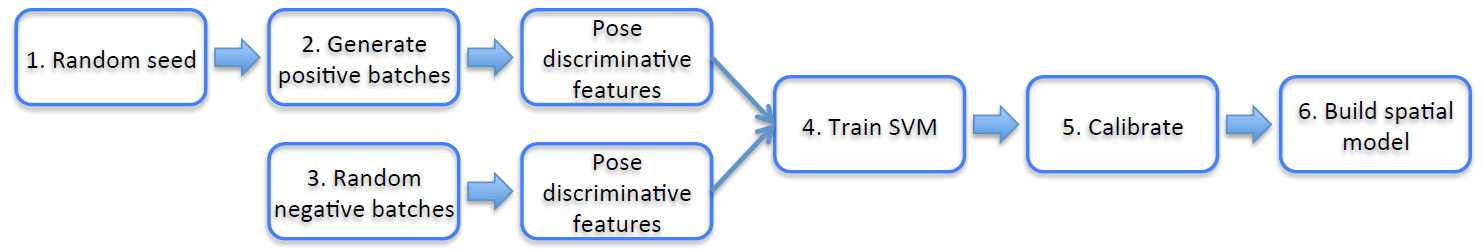
\includegraphics[scale=0.28]{cap2/class-pos}
\caption{Fasi addestramento classificatore poselet}
\label{class-pos}
\end{figure}

\subsection{Random Seed}
Il primo passo è quello di ottenere il \textit{Random Seed}: essa è una patch contenente un gruppo di keypoints in una particolare configurazione spaziale (faccia, due gambe, busto etc.) . Partendo dal Seed, cerchiamo nel training-set altre regioni che hanno la stessa configurazione spaziale dei keypoints. In questo caso è stato utilizzato come dataset PASCAL 2011\cite{pascal2011}, grazie alle annotazioni dei keypoints rilasciate su di esso\cite{pascal-keypoints}.\\

\subsection{Generazione campioni positivi}
Per trovare due regioni con la stessa configurazione di keypoints, utilizziamo la seguente distanza nello spazio 3D:

\begin{figure}[h]
\centering
  $d_s(r)=\sum_{i}w_s(i)||x_s(i)-x_r(i)||_2^2(1+h_{s,r}(i))$
  \caption{Distanza tra la configurazione di keypoint \textit{s} e \textit{r}}
\end{figure}

dove x$_s$(i)=[x,y,z] sono le coordinate 3D normalizzate dell'i-esimo keypoint di s. Il termine $w_s(i)\propto exp(-x_s(i)^2/(2\sigma ^2))$ è la Gaussiana con media nel centro della patch. $h_s,r(i)$ è una penalità basata sulla mancata corrispondenza di visibilità del keypoint \textit{i} nelle due regioni. Se il keypoint \textit{i} è visibile o invisibile in entrambe le regioni allora $h_s,r(i)=0$, altrimenti $h_s,r(i)=a, a>0$. Possiamo inoltre avere che il \textit{i}-th keypoint è presente in una regione ed assente in un altra: in questo caso il termine rispettivo è $w_s(i)b$ dove $(\sigma,\alpha,b,h)$ sono parametri fissati del modello.\\

\begin{figure}[h]
\centering
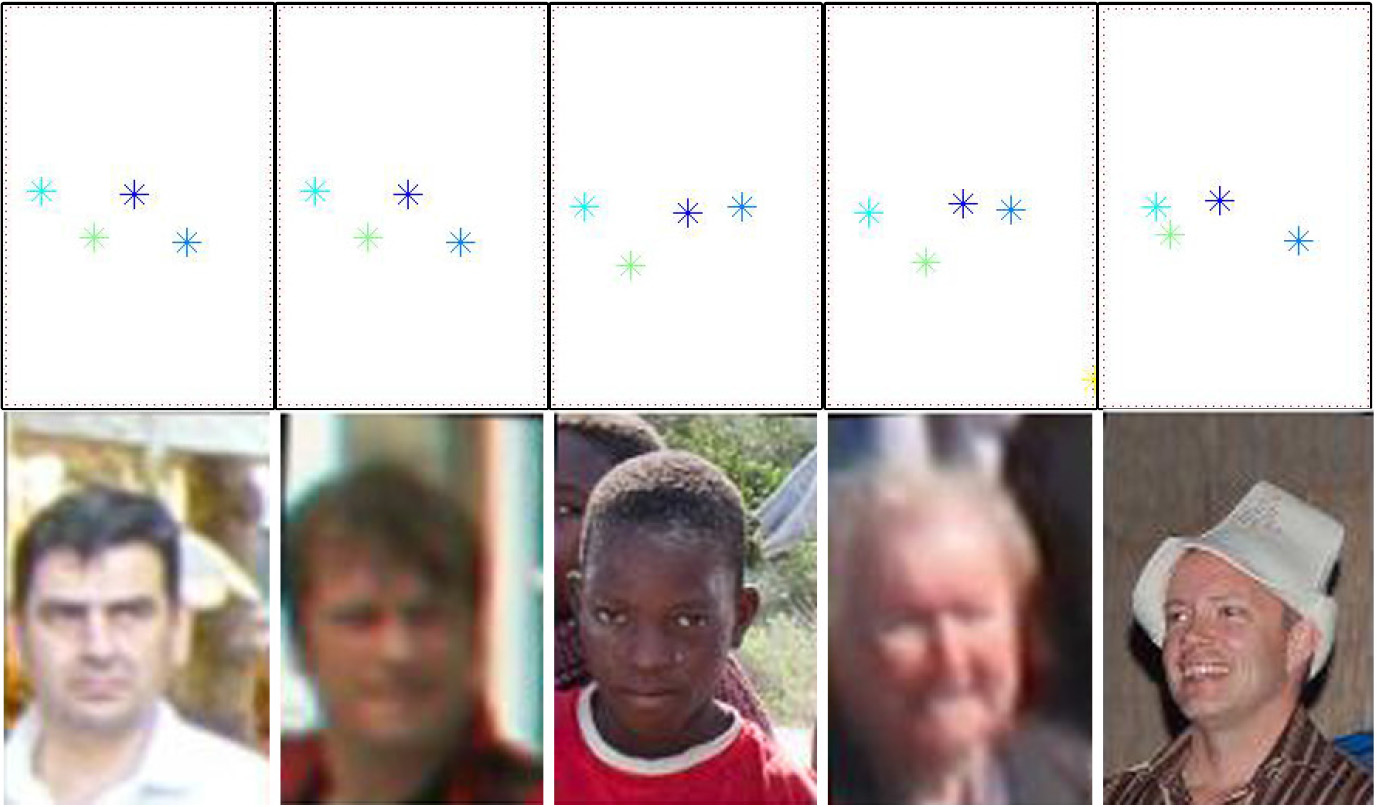
\includegraphics[scale=0.28]{cap2/face-keys}
\caption{Regioni con distribuzione dei keypoints simile}
\label{}
\end{figure}

\begin{figure}[h]
\centering
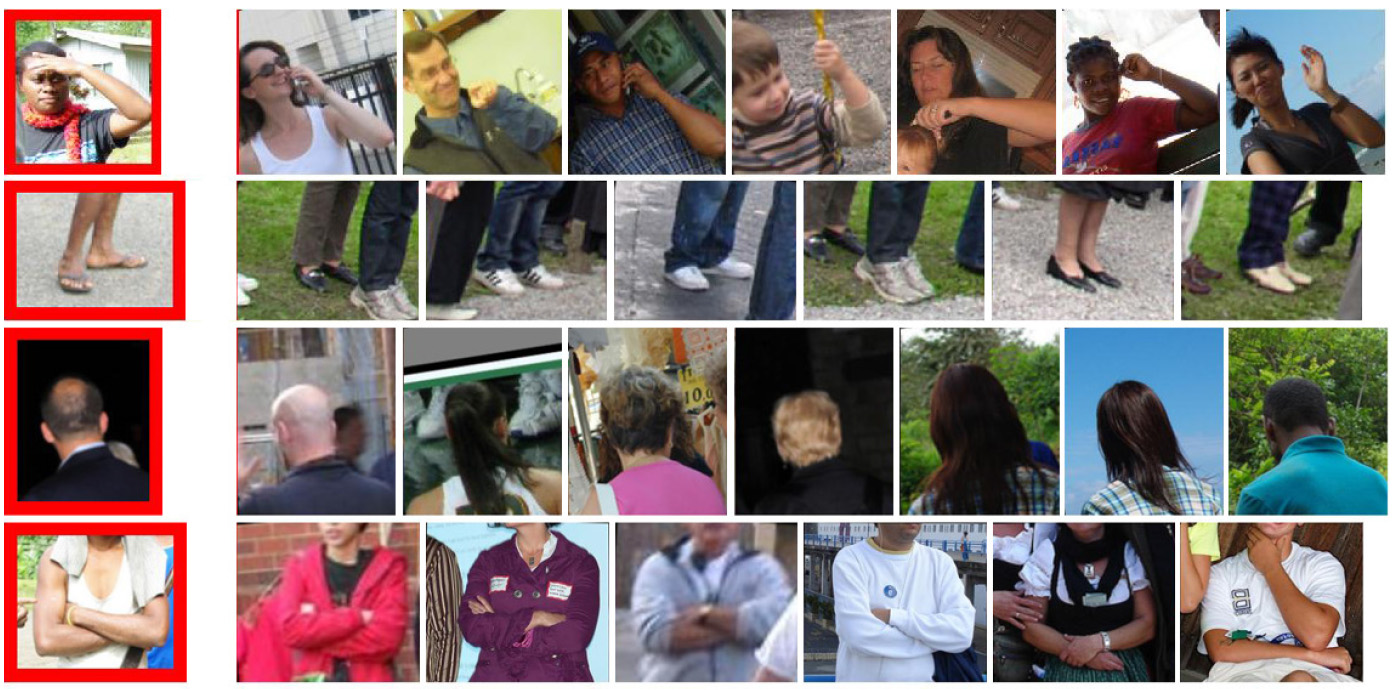
\includegraphics[scale=0.28]{cap2/pos-matches}
\caption{Sulla sinistra troviamo le regioni di query e i risultati ottenuti}
\label{}
\end{figure}

\subsection{Estrazione Caratteristiche}
Per estrarre le caratteristiche di ogni singola regione utilizziamo la Deep Net precedentemente addestrata. Eliminiamo dalla struttura l'ultimo layer (softmax layer) e utilizziamo il vettore di 256 dimensioni come vettore delle caratteristiche.

\subsection{Addestramento Classificatore}
Una volta scelto il Random Seed, collezionato regioni con configurazione di keypoints simile (campioni positivi) e scelto a caso campioni negativi, estraiamo per ogni regione il vettore delle caratteristiche e utilizziamo questi per addestrare un semplice classificatore SVM. Dopo aver addestrato per la prima volta l'SVM, applichiamo il classificatore ad una serie di regioni di immagini che non presentano persone all'interno. Prendiamo le regioni classificate come positive (sono dei falsi positivi), le aggiungiamo ai campioni negativi precedentemente collezionati e addestriamo nuovamente un SVM: questo procedimento permette di diminuire il tasso di rilevamento di falsi positivi.\\
Una volta addestrato il classificatore, eseguiamo la classificazione sui campioni positivi: l'SVM darà per ognuno di essi uno score. Per limitare il firing-rate di ciascun classificatore, selezioniamo il k-simo score e lo imponiamo come limite inferiore per il quale un campione viene classificato come positivo.\\
Dopo aver calibrato il firing-rate, diamo ad ogni classificatore uno score in dipendenza della sua bontà. Per fare ciò applichiamo il classificatore alle immagini che contengono le poselet-patch utilizzate per addestrare l'SVM ed etichettiamo le attivazioni-poselet individuate: essa sarà etichettata come positiva se l'intersection-over-union è almeno di 0.5 con la poselet patch presente nell'immagine. Una volta etichettate tutte le attivazioni-poselet e avendo i relativi score SVM, addestriamo un regressore logistico per convertire gli score in probabilità.

\begin{figure}[h]
 \centering
 \subfloat {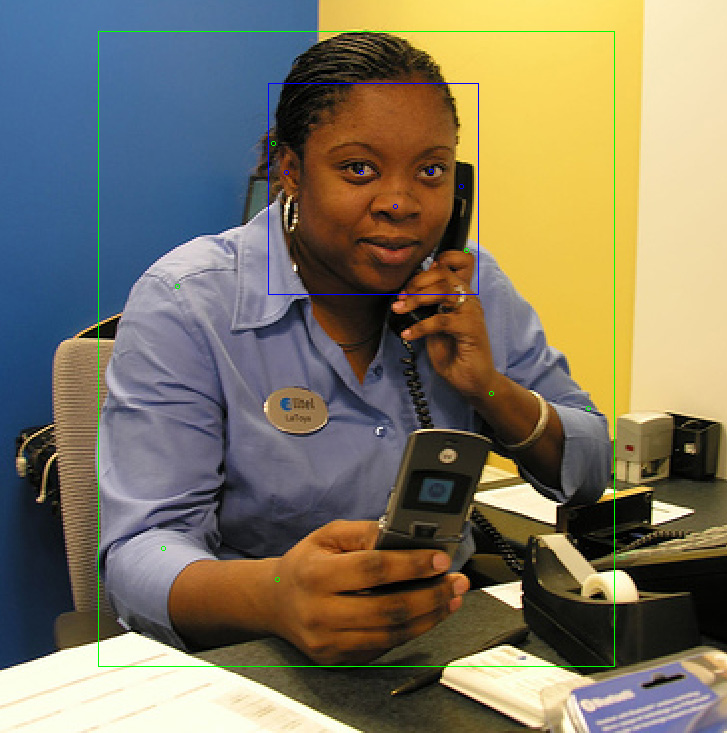
\includegraphics[scale=0.28]{cap2/image-patch}}
 \newline
 \subfloat {
\includegraphics[scale=0.7]{cap2/act-pos1}}
 \hspace{5mm}
 \subfloat {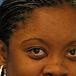
\includegraphics[scale=0.7]{cap2/act-pos2}}
 \hspace{5mm}
 \subfloat {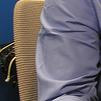
\includegraphics[scale=0.7]{cap2/act-neg}}
 \caption{In \textbf{alto} immagine del training set con relativa poselet-patch (in blu) e keypoints. In \textbf{basso} le prime due attivazioni-poselet sono etichettate come positive mentre la terza negativa}
 \end{figure}

A questo punto scegliamo un gruppo di classificatori poselet i quali avranno una buona probabilità di successo e si differenziano sulle zone del corpo da rilevare.\\

\subsubsection{Stima distribuzione keypoints e bounding boxes}
Nell'ultima fase di addestramento viene creato un modello spaziale: per ogni classificatore viene eseguita la stima della distribuzione dei keypoints e la predizione del bounding box.\\
Per la predizione dei keypoints eseguiamo il seguente procedimento: per ogni immagine utilizzata nella fase di addestramento dell'SVM, poniamo il centro del sistema di riferimento al centro della poselet-patch e calcoliamo la gaussiana relativa alla distribuzione dello spazio di ciascun keypoint: questo viene fatto per tutti i 20 keypoints anche se essi sono presenti fuori la poselet-patch o non presenti in qualche immagine. In questo modo avremo che se per esempio consideriamo la poselet-patch relativa alla faccia, avremo distribuzioni "piccate" in corrispondenza degli occhi e del naso.\\ \\
Per quanto riguarda la predizione del bounding box, portiamo sempre il centro del sistema di riferimento nel centro della poselet-patch e calcoliamo la media dei bounding boxes di tutte le immagini: il bounding box è definito dalle coordinate 2D dell'angolo alto-sinistro e basso-destro. In questo modo avremo che se consideriamo il bounding box predetto da un classificatore relativo alla poselet faccia, avremo che il lato superiore del bounding box sarà vicino al lato superiore della poselet-patch, mentre il lato inferiore sarà più distante (distanza piedi faccia): ovviamente se consideriamo il classificatore relativo alla poselet gambe è l'inverso.

\section{Funzionamento Classificatori}
In figura \ref{class-test} viene mostrato il procedimento per l'individuazione dei bounding box delle persone in immagini utilizzando i classificatori precedentemente addestrati.

\begin{figure}[h]
\centering
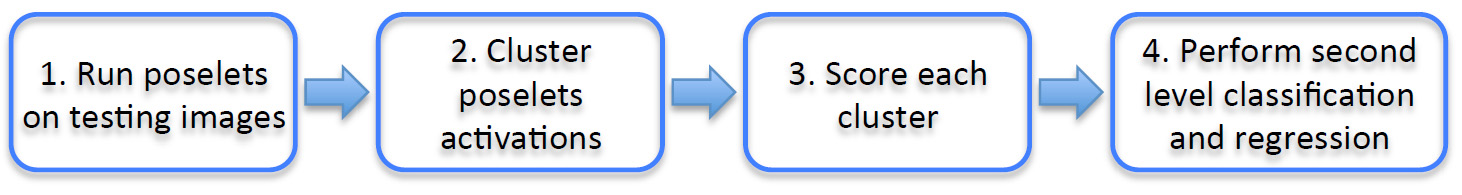
\includegraphics[scale=0.28]{cap2/class-test}
\caption{Rilevamento bounding boxes}
\label{class-test}
\end{figure}

Vengono estratte delle regioni dell'immagine di test tramite una finestra di dimensioni fissa 61x61 (dimensione input CNN) che si muove sull'intera immagine a varie scale: le regioni estratte dall'immagine scalata (scale diverso da 1) vengono ridimensionate a 61x61. Queste regioni vengono classificate con gli SVM relativi ai vari classificatori poselet e quindi vengono raccolte una serie di attivazioni.\\
Una volta ottenute le attivazioni, esse vengono clusterizzate col seguente approccio: prese le distribuzioni dei keypoint del classificatore relativo all'attivazione, le posizioniamo nello spazio immagine e inseriamo nello stesso cluster due attivazioni le quali distribuzioni hanno una KL-Divergence simmetrica minore di una certa soglia. Essa viene calcolata per ogni keypoint e viene effettuata la somma: in questo modo si considerano le distribuzioni dei singoli keypoints indipendenti tra loro.

\begin{figure}[h]
\centering
  $\sum \frac{ \sigma_1 + \Delta \mu ^2}{\sigma_2} + \frac{\sigma_2 + \Delta \mu^2}{\sigma_1} $
  \caption{KL-Divergence simmetrica}
\end{figure}

Ogni cluster avrà un proprio score che è dato dalla somma degli score delle attivazioni al suo interno. Per ciascun cluster portiamo nello spazio immagine le varie predizioni dei bounding boxes per ciascuna attivazione: la predizione finale del bounding box relativo al cluster sarà la media dei bounding boxes di tutte le attivazioni, ognuno pesato col suo score.\\

Nell'ultima fase i bounding boxes ottenuti vengono immessi in un'altra CNN, la R-CNN\cite{r-cnn}: essa permette la classificazione di una regione in differenti categorie, tra cui la categoria persona. 





